\documentclass[a4paper,10pt]{article}
\usepackage[utf8]{inputenc}

\usepackage{amstext, amsfonts, amsmath, amsbsy, amssymb}
\usepackage{url}
\usepackage[paper=a4paper,marginparwidth=0mm,marginparsep=0mm,margin=20.5mm,includemp]{geometry}
\usepackage{tikz}
\usepackage{blkarray}
\usepackage[colorlinks=true,linkcolor=blue,anchorcolor=blue,citecolor=blue,filecolor=blue,menucolor=blue,runcolor=blue,urlcolor=black]{hyperref} % For hyperlinks in the PDF
\usepackage[capitalise, noabbrev]{cleveref}

%Math symbols
\DeclareMathOperator{\Poisson}{Poisson}
\DeclareMathOperator{\Multinom}{Multinom}
\DeclareMathOperator{\logit}{logit}
\DeclareMathOperator{\cov}{cov}
\def\P{\mathbb{P}}
\def\E{\mathbb{E}}
\def\M{\boldsymbol{M}}
\def\I{{\cal I}}
\def\x{\boldsymbol{x}}
\def\d{\boldsymbol{d}}
\def\bnu{\mbox{\boldmath $\nu$}}
\def\bP{{\bf P}}
\def\R{{\bf R}}
\def\dd{\mathrm{d}}


\linespread{1.25}


%opening
\title{Inferring the presence of metabolites}

\begin{document}

\maketitle

\section{Idea and concept}
	
	We seek to infer the presence or absence of $M$ metabolites in $S$ species. We denote by $x_{sm}$ whether metabolite $m=1,\ldots,M$ is present ($x_{sm}=1$) or absent ($x_{sm}=0$) in species $s=1,\ldots,S$. To infer the full vector $\x=(x_{11}, \ldots, x_{1M},\ldots,x_{SM})$, we assume that related species share a similar set of metabolites and that metabolites related in their synthesis share a similar distribution across species. 
	Let $\P(x_{sm}=1|y_{sm})=y_{sm}$ be the probability with which metabolite $m$ is present in species $s$. We then assume that
	
	\begin{equation*}
	 \logit y_{sm} = \mu_m + \epsilon_{sm}
	\end{equation*}
	
	where $\mu$ is a metabolite-specific intercept and $\epsilon_{sm}$ is normally distributed with mean 0 and co-variance $\cov(\epsilon_{sm},\epsilon_{s'm'})=\alpha \sigma_{ss'} + \beta \sigma_{mm'}$ between each combination of species and metabolite. Here, $\sigma_{ss'}$ and $\sigma_{mm'}$ are known measures of covariance between species $s$ and $s'$ and between metabolites $m$ and $m'$, respectively, and $\alpha$ and $\beta$ are positive scalars.
	
	We consider two sets of data informative about $\x$: i) Presence-absence data obtained with mass-spectrometry and ii) presence-only reports of specific metabolites in specific specie. Let $\d_{sj}=(d_{sj1}, \ldots, d_{sjM})$ be the presence-absence vector of each metabolite $m$ obtained with mass-spectrometry run $j=1,\ldots,J_s$ performed on species $s$. Assuming a false-positive and false-negative error rates $\epsilon_{01}$ and $\epsilon_{10}$, respectively, we have
	
	\begin{equation*}
	 \P(\d_{sj}|\x, \epsilon_{01}, \epsilon_{10}) = \prod_m \left[ x_{sm}\left(\epsilon_{10}^{1-d_{sjm}}(1-\epsilon_{10})^{d_{sjm}}\right) + (1-x_{sm})\left( \epsilon_{01}^{d_{sjm}}(1-\epsilon_{01})^{1-d_{sjm}}\right)\right].
	\end{equation*}
	
	To model the presence only data, it must be put in relation to the expected research effort. Let $p_{sm}$ denote the known number of presence-only reports for metabolite $m$ in species $s$ and $n_{sm}$ the unknown number of research projects that aimed at discovering metabolite $m$ in species $s$. Assuming a false-positive and false-negative error rates $\pi_{01}$ and $\pi_{10}$, respectively, we have
	
	\begin{equation*}
	 \P(p_{sm}|n_{sm}, \pi_{01}, \pi_{10}) = 
	\end{equation*}
	
	
	We would have the covariance matrix such as :
	
	\begin{equation}
		\cov (\epsilon_{smt}, \epsilon_{s'm't'}) = \alpha \sigma_{ss'}^P + \beta \sigma_{mm'}^M + \gamma \sigma_{ss'}^E + \ldots
	\end{equation}
	
	With $P$ the phenotype between two species, $E$ an environment factor between two species and $M$ the TODO 

\section{DAG scratch}
\subsection{Test 1}
We assume that the probability of having a molecule in a species is the average presence of that molecule across all species $\mu_m$ plus a normally distributed error that depends on certain parameters $\alpha, \beta, \ldots$. 

From there, the LOTUS database and any result of MS depends on the set of molecules present in a species $\vec{\boldmath{x_s}}$. However we still have to take into account the fact that there can be an error of analysis on the MS $\epsilon_{m/z}$ that where $\epsilon_{m/z} = f(\epsilon_{01}, \epsilon_{10})$. 

Could we assume that as $j \rightarrow \infty$, then $d_{sj} \rightarrow \vec{\boldmath{x_s}}$ ?  TODO

According to Pierre-Marie LOTUS database is highly dependent on the research effort accorded to the specific molecule. He also said that error rate in the majority of LOTUS database is very low since most data is an actual isolation of the specific compound. Error rate of LOTUS database should then have little effect on the model. \\

	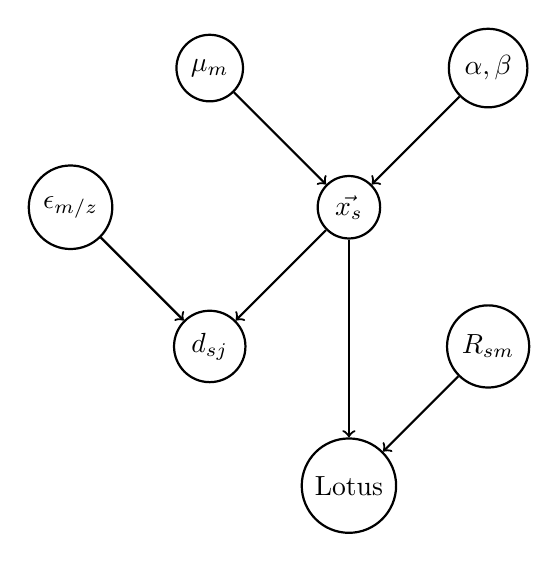
\begin{tikzpicture}[node distance={25mm}, thick, main/.style = {draw, circle}]
		\node[main] (1) {$d_{sj}$}; 
		\node[main] (2) [above left of=1] {$\epsilon_{m/z}$};
		\node[main] (7) [below right of=1] {Lotus};
		\node[main] (3) [above right of=7] {$R_{sm}$}; 
		\node[main] (4) [above right of=1] {$\vec{\boldmath{x_s}}$};
		\node[main] (5) [above left of=4] {$\mu_m$}; 
		\node[main] (6) [above right of=4] {$\alpha, \beta$};
		
		\draw[->] (5) -- (4);
		\draw[->] (6) -- (4);
		\draw[->] (4) -- (1);
		\draw[->] (2) -- (1);
		\draw[->] (4) -- (7);
		\draw[->] (3) -- (7);

	\end{tikzpicture} 


\subsection{Test 2}
\subsubsection{MS data}

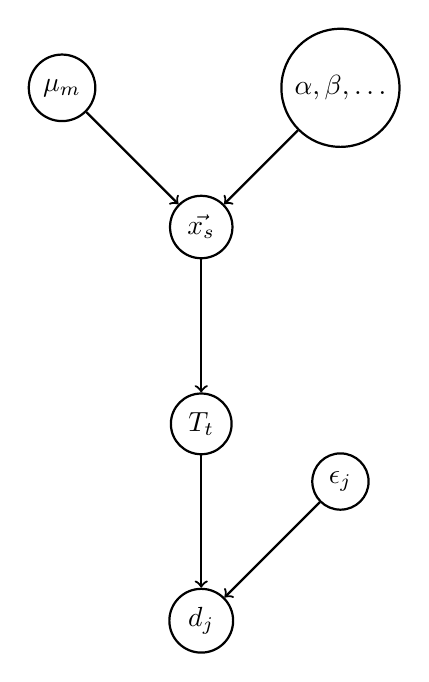
\begin{tikzpicture}[node distance={25mm}, thick, main/.style = {draw, circle}]
	\node[main] (1) {$\vec{\boldmath{x_s}}$};
	\node[main] (2) [above left of=1] {$\mu_m$};
	\node[main] (3) [above right of=1] {$\alpha, \beta, \ldots$};
	\node[main] (4) [below of=1] {$T_t$};
	\node[main] (5) [below of=4] {$d_j$};
	\node[main] (6) [above right of=5] {$\epsilon_j$};
	
	\draw[->] (2) -- (1);
	\draw[->] (3) -- (1);
	\draw[->] (1) -- (4);
	\draw[->] (4) -- (5);
	\draw[->] (6) -- (5);
\end{tikzpicture} 

With $\mu_m$ the average presence of a molecule across all species. $\alpha, \beta, \ldots$ the environmental variables (the error that is normally distributed across the mean). $x_s$ the molecule $x$ in species $s$. $T$ the tissue of species $s$. $d_j$ the mass spec data. The previous DAG can then be derived as the following. 
\begin{equation}
	P(\d | \mu_m, \alpha, \beta, \ldots) = \prod_{s=1}^{s}P(x_s|\mu_m, \alpha, \beta. \ldots) \prod_{t=1}^{t}\prod_{j=1}^{j}P(d_j | T_t, \epsilon_j)P(T_t | x_s)
\end{equation}

This is for one molecule. If we want to have for all the molecules we would have : 

\begin{equation}
	P(\d | \boldsymbol{\mu}, \alpha, \beta, \ldots) = \prod_{m=1}^{m}\prod_{s=1}^{s}P(x_s|\mu_m, \alpha, \beta. \ldots) \prod_{t=1}^{t}\prod_{j=1}^{j}P(d_j | T_t, \epsilon_j)P(T_t | x_s)
\end{equation}

Where do we go from here ? We search the probability of a molecule in a species give the data. We thus have $P(x|d) = \frac{P(x, d)}{P(d)}$. 

Where do we use Lotus DB ? Should it be our prior probability $P(x|d)$ ? 

\subsubsection{Error rate of MS}
We could have either a false positive meaning that the MS detects something that is not truly present in the species $0\rightarrow 1$ or a false negative meaning that a molecule is present in the sample but is not present in the data $1 \rightarrow 0$. 

Could this be viewed as a birth and death process ? If yes, this could be modelled with Kolmogorov forward- master equation: 
\begin{equation}
	\frac{dP_{ij}(t)}{dt} = \lambda_{j-1}P_{ij-1}(t) + \mu_{j+1}P_{ij+1}(t) - (\lambda_j + \mu_j)P_{ij}(t)
\end{equation}

\begin{itemize}
	\item With a Poisson process for birth ($0\rightarrow 1$) TODO ...
	\item HMM process ? 
\end{itemize}



\subsubsection{Error on Lotus DB}
Since the Lotus DB supposedly contains little to "no" errors, maybe we should also model as a Poisson process since error might occur but on rare occasions. 

The fact that Lotus doesn't contain many error is that each molecule present in the database, was isolated and analysed with either NMR or X-ray crystallography. Moreover, the latter techniques need to have a high amount of chemical extract so the probability that a compound is not present in the organism is close to 0 if not 0. However, not all entries in the database are made with these techniques so that is why we still need to account for that error in the model. 


\section{Formulation}
We seek to infer the presence or absence of $M$ metabolites in tissue $T$ in $S$ species. We denote by $x_{smt}$ whether metabolite $m=1,\ldots,M$ is present ($x_{smt}=1$) or absent ($x_{smt}=0$) in tissue $t = 1, \ldots T$ in species $s=1,\ldots,S$. We denote $\vec{x_{st}} = (x_{st1}, \ldots, x_{stM})$ the vector of molecules present in a tissue $T$ of a specific species $S$. 

Let us further denote $\vec{x_s} = (\vec{x_{s1}}, \ldots , \vec{x_{sT}}) = (x_{s11}, \ldots, x_{s1M}, x_{s21}, \ldots, x_{sTM})$ the vector of presence/absence of all molecules across all tissues for species $s$. 

We have two origins of data, mass spectrometry data and the Lotus database. We denote $d_{sj}$ the $j^{ \text th}$ mass spectrometry run for species $s$ and $\vec{L_s}$ all molecules assigned to species $s$ present in the LOTUS database. Finally we define $R$, a function representing the research effort produced for either a species $s$ or a specific molecule $m$. We also define $\vec{\epsilon_j}$ a vector of error that is specific for each mass-spectrometry run. 

A DAG of the model can be seen in \cref{fig:DAG_model}. $\vec{\mu}$ being the vector of the average presence/absence of each molecule across all species and $\vec{\alpha}$ represents the vector of all known measures of covariates between species and molecules. 

Since the tissue specific origin of a molecule is not known in the LOTUS database \cite{rutzLOTUSInitiativeOpen2022}, we denote $$P(\vec{L_S} | \vec{x_s}, R) = P(\vec{L_s} | \vec{\xi_s}, \vec{R}), $$ with $\vec{\xi_s} = (\xi_{s1}, \ldots, \xi_{sM} )$ the vector of presence/absence of all molecules $M$ in species $s$. Furthermore, $\xi_{sm} = min(1, \sum_{t}^{T} x_{smt})$ the minimum between $1$ and the sum of presence or absence of a molecule across all tissues. 

\begin{figure}
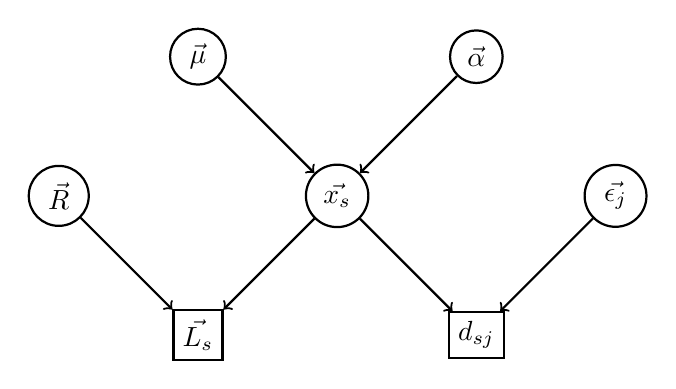
\begin{tikzpicture}[node distance={25mm}, thick, main/.style = {draw, circle}]
	\node[main] (1) {$\vec{\boldmath{x_s}}$};
	\node[main] (2) [above left of=1] {$\vec{\mu}$};
	\node[main] (3) [above right of=1] {$\vec{\alpha}$};
	\node[draw] (4) [below right of=1] {$d_{sj}$};
	\node[draw] (5) [below left of=1] {$\vec{L_s}$};
	\node[main] (6) [above right of=4] {$\vec{\epsilon_j}$};
	\node[main] (7) [above left of=5] {$\vec{R}$};
	
	\draw[->] (2) -- (1);
	\draw[->] (3) -- (1);
	\draw[->] (1) -- (4);
	\draw[->] (1) -- (5);
	\draw[->] (6) -- (4);
	\draw[->] (7) -- (5);
\end{tikzpicture} 
\caption{Potential DAG of the model.}
\label{fig:DAG_model}
\end{figure}

We can also denote $\vec{R} = (R_{11}, \ldots, R_{1M}, R_{21}, \ldots, R_{SM})$ the vector of \textit{research effort} of all molecules across all species. 

The probability of having a molecule present in the LOTUS database not only depends on the presence/absence of that molecule in a species but also on the research effort done for a specific molecule or species. We thus have $R_{sm} = f(n_s, n_m)$ with $R_{sm} \in [0,1]$ and where $n_s$ and $n_m$ are the number of scientific papers that relate respectively the species and the molecules of interest. We thus have the following matrix : \\

\begin{blockarray}{cccc}
	& $L_{sm} = NA$ & $L_{sm} = 1$ \\
	\begin{block}{c(ccc)}
		$x_{sm}=0$ & $1$ & $0$  \\
		$x_{sm}=1$ & $1-R_{sm}$ & $R_{sm}$ \\
	\end{block}
\end{blockarray}

Tissue of origin is usually known in mass spectrometry analysis. From \cref{fig:DAG_model}, we have, $P(d_{sj} | \vec{x_s}, \vec{\epsilon_j}) = P(d_{sj} | \vec{x_{st(d_{sj})}}, \vec{\epsilon_j}) $ where $t(d_{sj})$ reflects the tissue from which mass spectrometry run $j$ in species $s$ was sampled. 

We thus have: 

\begin{equation}
	P(\d, \x, \boldsymbol \mu, \boldsymbol \alpha )  = P(\boldsymbol{\mu})P(\boldsymbol{\alpha}) \prod_{s=1}^{S} P(\vec{x_s} | \boldsymbol{\mu}, \boldsymbol{\alpha}) \prod_{j=1}^{J} P(d_{sj} | \vec{x_{st(d_{sj})}}, \vec{\epsilon_j})
\end{equation}

Similarly, for LOTUS database we have :

\begin{equation}
	P(\L, \x, \boldsymbol \mu, \boldsymbol \alpha ) = P(\boldsymbol{\mu})P(\boldsymbol{\alpha}) P(\R) \prod_{s=1}^{S} P(\vec{x_s} | \boldsymbol{\mu}, \boldsymbol{\alpha}) P(L_s | \vec{x_s}, \R)
\end{equation}


\bibliographystyle{unsrturl}
\bibliography{/Users/Marco/BibTex/BibTex}

\end{document}
